\section{Random Variables}

\subsection{Introduction}

A random variable is a function that maps elements from a sample space to any real number: $X : S\to\mathbb{R}$. It is usually denoted by $X, Y, Z, N$. Let $s$ be a member of a sample space $S$, if $s$ is picked up by probability function $P$ then random variable $X(s)$ returns a real number. A random variable can either be discrete or continuous. \\

A discrete random variable only takes finite (or countably infinite) $m$ values: $\{x_1, x_2, \dots, x_m\}$. The sample space is broken into discrete partitions.

\begin{figure}[H]
	\centering
	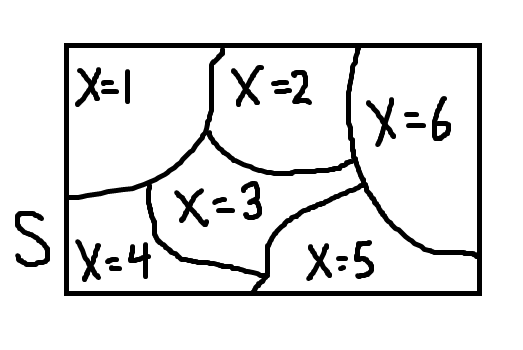
\includegraphics[width=120mm]{4.png}
	\caption{Example of a discrete R.V.}
\end{figure}

On the other hand, a continuous random variable can take infinitely many values. One such example is a coordinate on the x-axis which is represented by a real number: $X(x)=x$. \\

The probability when a random variable takes a certain value is denoted by $P(X=a)$ which is the shortcut for writing $P(\{s \in S \mid X(s)=a\})$. Ranges are also allowed: $P(X\le a)=P(\{s \in S \mid X(s)\le a\})$.

\begin{texample}
	You roll two dice. Find probabilities of each sum. What is the probability of rolling $30$ or $\pi$? \\
	
	The sample space for two dice rolls is $S=\{(a,b) \mid a,b \in \{1, 2, \dots, 6\}\}$. The random variable relevant to this problem is $X((a,b))=a+b$. Below are probabilities for each possible sum.
	
	\begin{align*}
		&P(X = 2) = P((1, 1)) = \frac{1}{36} \\
		&P(X = 3) = P((1, 2), (2, 1)) = \frac{2}{36} \\
		&P(X = 4) = P((1, 3), (2, 2), (3, 1)) = \frac{3}{36} \\
		&P(X = 5) = P((1, 4), (2, 3), (3, 2), (4, 1)) = \frac{4}{36} \\
		&P(X = 6) = P((1, 5), (2, 4), (3, 3), (4, 2), (5, 1)) = \frac{5}{36} \\
		&P(X = 7) = P((1, 6), (2, 5), (3, 4), (4, 3), (5, 2), (6, 1)) = \frac{6}{36} \\
		&P(X = 8) = P((2, 6), (3, 5), (4, 4), (5, 3), (6, 2)) = \frac{5}{36} \\
		&P(X = 9) = P((3, 6), (4, 5), (5, 4), (6, 3)) = \frac{4}{36} \\
		&P(X = 10) = P((4, 6), (5, 5), (6, 4)) = \frac{3}{36} \\
		&P(X = 11) = P((5, 6), (6, 5)) = \frac{2}{36} \\
		&P(X = 12) = P((6, 6)) = \frac{1}{36}
	\end{align*}
	
	Notice that the total probability adds up to one
	
	$$\sum_{n=2}^{12} P(X=n)=1$$
	
	As for $30$ and $\pi$, the probability is zero.
\end{texample}

\subsubsection{Commutative Distribution Function}

We conclude this section with brief words on commutative distribution functions (CDF). CDF for a random variable $X$ is defined as

$$F_X (a)=P(X\le a)$$

for all $a$ values. In other words, $F_X(a)$ is the sum of probabilities from $-\infty$ to $a$. \\

The basic properties of $F_X(a)$ are:

\begin{enumerate}[i]
	\item $0 \le F_X(a) \le 1$
	\item $F_X(a_1) \le F_X(a_2)$ for $a_1 < a_2$
	\item $\displaystyle \lim_{a\to-\infty} F_X(a)=0$
	\item $\displaystyle \lim_{a\to\infty} F_X(a)=1$
\end{enumerate}

The last two properties indicate the function $F_X(a)$ is monotone increasing. \\

We can calculate probabilities from CDFs using the following relations:

\begin{enumerate}[i]
	\item $P(a<X\le b)=F_X(b)-F_X(a)$
	\item $P(X>a)=1-F_X(a)$
\end{enumerate}

Notice that the first property vaguely resembles the fundamental theorem of calculus. We will see later that CDFs are what we get when we integrate probability density functions (PDF). \\

\subsection{Discrete Random Variables}

Since discrete random variables take a finite number of values, their CDF $F_X(a)$ changes in discrete steps for each value and are constant between jumps (think of stairs). Before we go further, we need to discuss probability mass functions (PMF) first.

\subsubsection{Probability Mass Function}

PMFs $p_X(x)$ are like bar charts used for calculating probability involving discrete random variables. They are defined in such a way that

$$p_X(a)=P(X=a)$$

for a discrete random variable $X$ which takes the following values: $\{x_1, x_2, \dots, x_m\}$. They satisfy the following properties:

\begin{enumerate}[i]
	\item $p_X (x_i) \ge 0$ for all $i$
	\item $\sum_i^m p_X (x_i)=1$
\end{enumerate}

$F_X(a)$ for a discrete variable can be found using: $F_X(a)=P(X\le a)=\sum_{x_i\le a} p_X(x_i)$. \\

We either use $p_X (x)$ or $F_X (a)$ to specify a discrete random variable. We will take a look at some special discrete random variables.

\subsubsection{Bernoulli Random Variable}

Bernoulli random variable $X \sim \Bern (p)$ is useful for experiments involving binary outcomes, like ``pass'' and ``fail'' or ``positive'' or ``negative.'' $X$ either takes $0$ or $1$ where $0$ represents ``failure'' and $1$ represents ``success.''

\begin{figure}[H]
	\centering
	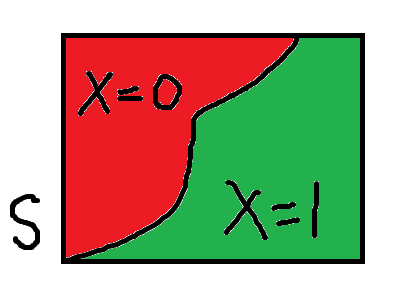
\includegraphics[width=80mm]{5.png}
	\caption{Bernoulli Random Variable}
\end{figure}

Suppose the probability for ``success'' is $p$, PMF for $X$ is given by:

$$p_X(n)=P(X=n)=p^n(1-p)^{1-n}$$

where $p_X\in[0,1]$ and $n=0,1$, or alternatively:

$$p_X(1)=P(X=1)=p$$
$$p_X(0)=P(X=0)=1-p$$

The CDF $F_X(a)$ is given by

$$
F_X(a)=
\begin{cases} 
	0 & a<0 \\
	1-p & 0\le a<1 \\
	1 & x \ge 1
\end{cases}
$$

\begin{figure}[H]
	\centering
	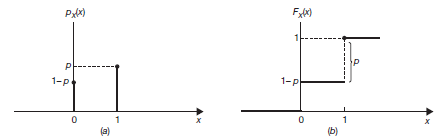
\includegraphics[width=120mm]{6.png}
	\caption{Bernoulli Distribution}
\end{figure}

\subsubsection{Geometric Random Variable}

Suppose you are carrying out some number of Bernoulli trials that has a success rate of $q$ each time independently. You want to calculate the probability that after $n$ tries you achieved your first success. The probability is calculated as follows:

$$P(X=n)= \underbrace{ (1-q)(1-q) \cdots (1-q) }_{ \text{$n-1$ times} } q=(1-q)^{n-1} q$$

The suitable random variable for this problem is the geometric random variable $X \sim \Geom (q)$. The possible values of $n$ are $1, 2, \dots$. Its PMF is given by

$$p_X(n)=P(X=n)=(1-q)^{n-1} q$$

where $p\in(0,1]$ and $n=1, 2,\dots$. Its CDF is given by

$$F_X(a)=1-(1-q)^a$$

where $a=1, 2,\dots$. \\

Note that this random variable is still discrete even though it can take infinitely many values because they take countably infinite integer values.

\begin{figure}[H]
	\centering
	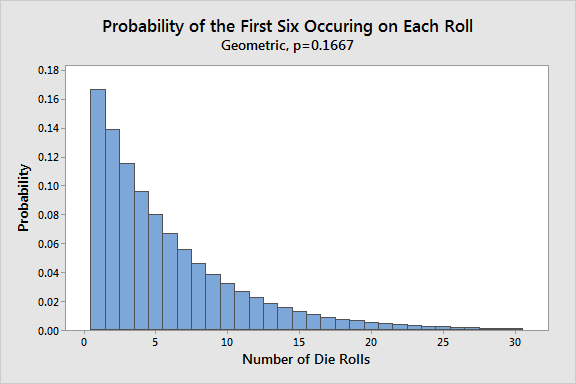
\includegraphics[width=120mm]{7.png}
	\caption{Example Geometric PMF}
\end{figure}

\begin{figure}[H]
	\centering
	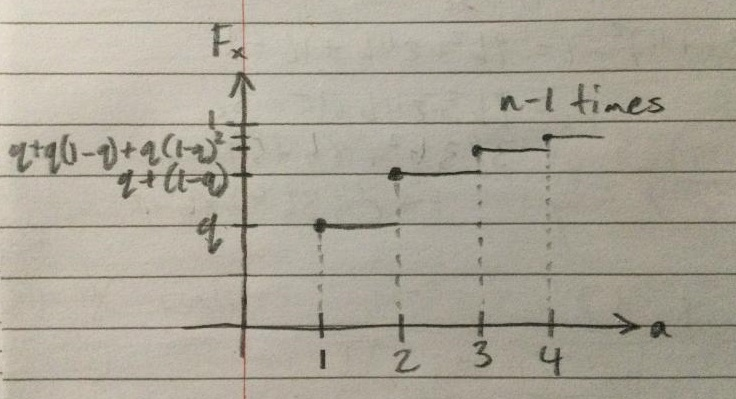
\includegraphics[width=120mm]{8.jpg}
	\caption{Geometric CDF}
\end{figure}

For a discrete random variable, $\sum_i p_X (x_i)=1$ but for geometric random variable which is countably infinite,

$$\sum_{n=1}^\infty p_X(n) = \sum_{n=1}^\infty (1-q)^{n-1} q = 1$$

It can be proved using the formula for infinite geometric series:

\begin{align*}
	\sum_{n=1}^\infty (1-q)^{n-1} q &= q \sum_{n=1}^\infty (1-q)^{n-1} \\
	&= q \sum_{n=0}^\infty (1-q)^{n} \\
	&= q\frac{1}{1-(1-q)} = 1
\end{align*}

A geometric random variable has something called \textit{memoryless property}. The idea is that if an experiment failed $n$ times then the probability that $m$ additional failures will happen is the same as the probability that the experiment failed $m$ times at the start. It indicates that the probability does not depend on past events. This property can be summarized by the below equation:

$$P(X>n+m\mid X>n)=P(X>m)$$

Explicit example: Consider an experiment of coin tosses and you happened to flip $5$ tails in a row and with that information, the probability of getting an additional $2$ tail is exactly the same as the probability of getting $2$ tails. \\

Also, note that

$$P(X>n+m\mid X>n)=P(X>n+m)$$

is not always true unless events $X>n+m$ and $X>n$ are independent (ie. $P(X>n)=1$). \\

\begin{figure}[H]
	\centering
	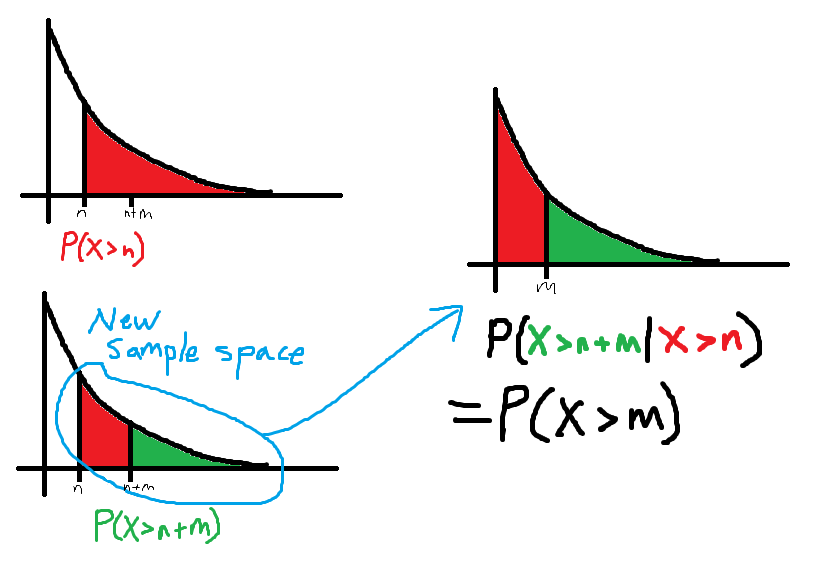
\includegraphics[width=120mm]{9.png}
	\caption{Visualization for Memoryless Property on PDF}
\end{figure}

To prove the memoryless property, consider

\begin{align*}
	P(X>n)&=\sum_{a=n+1}^\infty p_X(a)\\
	&=\sum_{a=n+1}^\infty (1-q)^{a-1}q\\
	&=q(1-q)^n\sum_{a = 0}^\infty (1-q)^a\\
	&=(1-q)^n\sum_{a = 0}^\infty (1-q)^aq
	\intertext{Since the sum of the whole PMF is one,}
	&=(1-q)^n
\end{align*}

Applying the formula for conditional probability,

\begin{align*}
	P(X>n+m\mid X>n)&=\frac{P(X>n+m\cap X>n)}{P(X>n)}\\
	&=\frac{(1-q)^{n+m}}{(1-q)^n}\\
	&=(1-q)^m=P(X>m)
\end{align*}

\subsubsection{Binomial Random Variable}

Binomial random variable $X\sim\Bin(n,q)$ describes the number of successes if an experiment is repeated $n$ times, each with success rate $q$. Each experiment must be independent of each other. Examples of such experiments like coin flips or any experiment with binary outcomes. \\

Its PMF is given by

$$p_X(k)=P(X=k)={n \choose k} q^k(1-q)^{n-k}$$

where $k=0, 1, 2, \dots, n$. This formula gives the probability of getting exactly $k$ successes out of $n$ trials. \\

\begin{figure}[H]
	\centering
	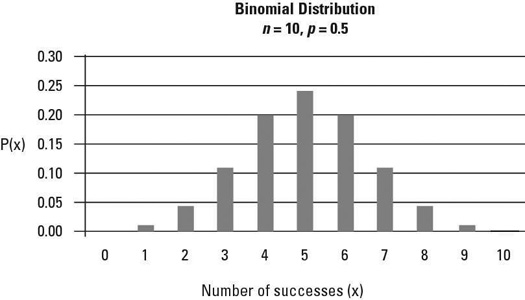
\includegraphics[width=120mm]{10.jpg}
	\caption{Example binomial PMF}
\end{figure}

The below example will build intuition on where the formula came from.

\begin{texample}
	Consider an unfair coin, let the probability of getting $H$ on a single toss be $0.6$ and the probability of getting $T$ is $0.4$. Find (1) the probability of obtaining the sequence $THHTTTHT$ (exactly, in this order) (2) the probability that a sequence of eight coin tosses would have $5$ tails and $3$ heads in any order. \\
	
	(1) Coin toss events are independent of each other. The probability will be calculated as follows $0.4\cdot0.6\cdot0.6\cdot0.4\cdot0.4\cdot0.4\cdot0.6\cdot0.4=0.6^30.4^5=0.00221$. By symmetry, this is the same as the probability of getting the sequence $TTTTTHHH$ (or any other arrangements involving $3$ heads and $5$ tails) in exact order. \\
	
	(2) The probability of getting $5$ tails and $3$ heads in any order can be calculated using the addition law for disjoint events:
	
	\begin{align*}
		P(\text{$3$ heads})&=P(\{THHTTTHT\}) + P(\{THTHTTTH\}) \\
		&\quad+ P(\{TTHTHHTT\}) + \cdots \\
		&\quad + P(\{\text{other arrangements of $3H$ and $5T$}\})
	\end{align*}
	
	In this case, we need to find the number of ways to permute $5$ tails and $3$ heads which is given by $\binom{8}{3}=56$. Using our answer to (1), the probability is therefore:
	
	$$P(\text{$3$ heads})=56\cdot0.00221=0.12386$$
\end{texample}

The total probability of binomial PMF is indeed one:

$$\sum_{k=0}^{n} p_X(k) = \sum_{k=0}^{n} {n \choose k} q^k(1-q)^{n-k} = (q+(1-q))^n=1^n=1$$

\begin{texample}
	Using the same unfair coin from the previous example, define a score to be (number of Heads) / (number of tosses). Find the probability that the score is between $0.4$ and $0.8$ when $N=9$ coins are tossed. What is the answer if $N$ is very large? \\
	
	To get the score between $0.4$ and $0.8$, we need to get $4$ to $7$ heads. So the probability is
	
	\begin{align*}
		P(\text{score between 0.4 and 0.8})&=P(\text{4 or 5 or 6 or 7 heads}) \\
		&= P(\text{4 heads})+P(\text{5 heads}) \\
		&\quad + P(\text{6 heads})+P(\text{7 heads}) \\
		&= \sum_{k=4}^7 \binom{9}{k}0.6^k0.4^{9-k} \\
		&= 0.8301
	\end{align*}
	
	If $N$ is very large, the probability will reach $1$.
\end{texample}

\begin{texample}
	You roll $5$ dice and what is the probability that you get $3$ sixes? \\
	
	Let $X$ denote the number of sixes showing. There is $\frac16$ chance to roll six and $\frac56$ chance to roll other numbers. The probability of getting $3$ sixes is
	
	$$P(X=3)={5\choose3}\left(\frac16\right)^3\left(\frac56\right)^2=0.032$$
\end{texample}

\subsubsection{Poisson Random Variable}

Poisson random variable $X\sim\Pois(\lambda)$ can be used to find the probability of some number of events happening in some specified time period given that the event happens at some constant rate of $\lambda$ and the events occur independently. Its PMF is given by

$$p_X(n)=P(X=n)=e^{-\lambda}\frac{\lambda^n}{n!}$$

where $n=0,1,2,\dots$. It calculates the probability that $n$ events will happen at the specified time period. The parameter $\lambda>0$ can be thought as the mean number of event occurrences happening in the given time period or rate (units: occurrences per time). This PMF works because

$$\sum_{n=0}^\infty p_X(n) = \sum_{n=0}^\infty e^{-\lambda}\frac{\lambda^n}{n!} = e^{-\lambda} \sum_{k=0}^\infty \frac{\lambda^n}{n!}=e^{-\lambda}e^\lambda=1$$

The probability that $n$ events will happen in time interval $t$ given the event rate $r$ (the parameter is $\lambda=rt$) is

$$P(X=n)=e^{-rt}\frac{(rt)^n}{n!}$$

The possible examples of this random variable is not limited to the number of typos in a book, the number of radioactive decays in some time interval, and the number of people who failed exams. \\

Compared to binomial random variables which count discrete occurrences among discrete trials, the Poisson random variables count discrete occurrences among a continuous domain.

\begin{figure}[H]
	\centering
	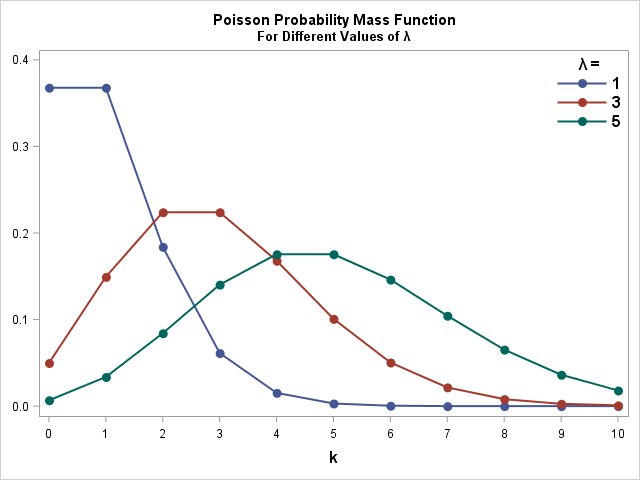
\includegraphics[width=100mm]{11.png}
	\caption{Poisson PMFs for different values of $\lambda$. The PMF with $\lambda=3$ is peaked at $k=3$ which makes sense because events with the mean number of occurrences $\lambda=3$ per time frame of $10$ will most likely happen at $3$ times out of $10$.}
\end{figure}

When the number of trials $n$ of a binomial random variable approaches infinity and the probability of success $p$ approaches zero, it can be approximated with Poisson random variable with parameter $\lambda=pn$. This is a very robust approximation. \\

Consider a binomial random variable $X\sim\Bin(n,q)$, applying $\lambda=pn$ to its distribution gives

\begin{align}
	P(X = k) &= {n \choose k}p^k(1-p)^{n-k} \\
	&=\frac{n(n-1)(n-2)\cdots(n-k+1)}{k!}\frac{\lambda^k}{n^k}\left(1-\frac{\lambda}{n}\right)^{n-k} \\
	&=\frac{n(n-1)(n-2)\cdots(n-k+1)}{n^k}\frac{\lambda^k}{k!}\left(1-\frac{\lambda}{n}\right)^n\left(1-\frac{\lambda}{n}\right)^{-k}
\end{align}

Now as $n \to \infty$ and $p \to 0$, we have

$$\frac{n(n-1)(n-2)\cdots(n-k+1)}{n^k} \approx 1 \quad \left(1-\frac{\lambda}{n}\right)^n \approx e^{-\lambda} \quad \left(1-\frac{\lambda}{n}\right)^{-k} \approx 1$$

This gives

$$P(X = k) \approx \frac{\lambda^k}{k!}e^{-\lambda}$$

We get the Poisson approximation of $X$ as expected. We can see that Poisson random variables are great for modelling occurrences of events that could happen a very large number of times but happen rarely. Sometimes Poisson is preferred over binomial as they make calculations easier.

\begin{texample}
	Birthday problem revisited: In a room of $n$ people, approximate the probability that at least $2$ people share the same birthday. \\
	
	We will take a slightly different route from the last time. Imagine going over every possible pair of $n$ people and marking it off as a success when both of them share the same birthday. The probability of success happening is $\frac{1}{365}$. There are ${n \choose 2}$ possible pairs. \\
	
	We can employ the Poisson approximation here. Let $X\sim\Pois(\lambda)$ denote the number of pairs who share the same birthday where the average number of successful pairs is $\lambda={n \choose 2}\frac{1}{365}$. The probability that at least one pair share the same birthday is $P(X>0)=1-P(X=0)$ where $P(X=0)$ is the probability that none of the pairs share the same birthday. We get
	
	$$P(X>0)=1-e^{-\lambda}=1-\exp\left( -{n \choose 2}\frac{1}{365} \right)$$
	
	As an example, suppose $n=23$, $P(X>0)=0.5$. \\
	
	The Poisson approximation can be generalized to more than two people. If we want to find the probability that at least three people share the same birthday, we only need modify the Poisson parameter which will be $\lambda={n \choose 3}\frac{1}{365^2}$ since we now need to choose three people and there is $\frac{1}{365^2}$ chance that three of them share the same birthday. \\
	
	As a side note, binomial distribution cannot be used in this problem because it only works when events are independent which is not the case here. The probability of a person having a different birthday dependent on another person's birthday. But it is still ``possible'' to apply binomial distribution here since the Poisson's approximation works. For example if $n=23$, the probability is
	
	$$P(X>0)=1-\left({n \choose 0} \left( p \right)^0 \left( 1-p \right)^{n}\right)=0.50048$$
	
	where $n={23 \choose 2}$ and $p=\frac{1}{365}$. It is close enough to Poisson's approximation. This is only because $n$ is large and $p$ is small.
\end{texample}

\begin{texample}
	You repeat an experiment $1000$ times, each with an independent success rate of $\frac{1}{500}$. Find the probability of getting at most two successes. \\
	
	Denote $n=1000$ and $p=\frac{1}{500}$. One can use a binomial random variable to find probability:
	
	\begin{align*}
		P(\text{at most 2 success}) &= P(\text{0 success})+P(\text{1 success})+P(\text{2 success}) \\
		&= \sum_{k=0}^2 {n\choose k} p^k (1-p)^{n-k} \\
		&= 0.67668
	\end{align*}
	
	An even better way to solve is to approximate using a Poisson random variable $X\sim\Pois(\lambda)$ where $\lambda=pn=2$. This gives
	
	\begin{align*}
		P(X \le 2)&=P(X=0)+P(X=1)+P(X=2) \\
		&=e^{-\lambda}+e^{-\lambda}\frac{\lambda}{1}+e^{-\lambda}\frac{\lambda^2}{2}=5e^{-2} \\
		&=0.67668
	\end{align*}
	
	This approximation works well because $n$ is large and $p$ is small.
\end{texample}

\subsubsection{Expectation Value}

The expectation value of a discrete random variable $X$ with corresponding PMF $p_X(x)$ is

$$E[X]=\sum_i x_i p_X(x_i)$$

It is the weighted average of all possible values $X$ can take $x_i$. It is denoted by either $E[X]$ (or simply $EX$) or $\langle X \rangle$. It is different from the average which is the mean result obtained after repeating an experiment for some number of times. But the average will become the expectation value if the experiment is repeated for infinite number of times (law of large numbers).

\begin{texample}
	Let $X$ represent the outcome of a dice roll. Find its expectation value. \\
	
	The possible values of $X$ are $x_i=1, 2, \dots, 6$ and the probability of rolling one of these values is $p_X(x_i)=\frac16$ so the expectation value is:
	
	$$E[X]=\sum_{i=1}^6 x_i p_X(x_i)=1\frac16+2\frac16+3\frac16+4\frac16+5\frac16+6\frac16=3.5$$
	
	It represents the average result you get if you roll the dice for infinite number of times.
\end{texample}

The expectation value for a Bernoulli random variable can be calculated in a straightforward manner as follows:

$$E[X\sim\Bern(p)]=1p+0(1-p)=p$$

For geometric random variables, consider

$$f(x)=\sum_{n=0}^\infty x^n = \frac{1}{{1-x}} \quad f'(x)=\sum_{n=0}^\infty nx^{n-1} = \left(\frac{1}{{1-x}}\right)^2$$

Let $x=1-q$,

$$f'(1-q)=\sum_{n=0}^\infty n(1-q)^{n-1} = \frac{1}{q^2}$$

multiplying both sides by $q$ gives

$$q\sum_{n=0}^\infty n(1-q)^{n-1} = \sum_{n=0}^\infty nq(1-q)^{n-1} = \frac{1}{q}$$

This gives the closed formula for the expectation value of geometric random variables (remember that they start from $n=1$, not $n=0$):

$$E[X\sim\Geom(q)]=\sum_{n=1}^\infty nq(1-q)^{n-1}=\frac1q$$

For binomial random variables, consider

$$\sum_{k=0}^n x^k p(k) = \sum_{k=0}^n {n \choose k} (qx)^k (1-q)^{n-k}=(1-q+qx)^n$$

taking a derivative with respect to x gives

$$\sum_{k=0}^n kx^{k-1} p(k) =n(1-q+qx)^{n-1}q$$

setting $x=1$,

$$\sum_{k=0}^n k p(k) =n(1)^{n-1}q=nq$$

This gives the expectation value for a binomial random variable

$$E[X\sim\Bin(n,q)]=nq$$

Finally, for Poisson random variables, we start with

$$f(x)=\sum_n e^{-\lambda} \frac{\lambda^n}{n!}x^n$$

applying the Taylor expansion for $e^\lambda$,

$$f(x)=e^{-\lambda}e^{\lambda x}=e^{\lambda x-\lambda}$$

the derivative of $f(x)$ is

$$f'(x)=\lambda e^{\lambda x-\lambda}$$

Notice that $f(1)=1$, which is the total probability of Poisson PMF, and $f'(1)=\lambda$. This gives a Poisson random variable expectation

$$E[X\sim\Pois(\lambda)]=\lambda$$

We see that the general strategy for finding closed-form expression for expectation is to start with a generating function of the following form

$$f(x)=\sum_n x^n p(n)$$

where $x$ takes values in $\mathbb{N}$. $f(1)=1$ represents the sum of probabilities. The derivative of this function is

$$f'(x)=\sum_n nx^{n-1} p(n)$$

$f'(1)$ usually gives the expectation value.

\subsection{Continuous Random Variables}

A random variable $X$ is said to be continuous if there exists a function $f_X(x)$ defined for all real numbers $x\in\mathbb{R}$ such that

$$P(X\in B)=\int_B f_X(x) dx$$

where $B$ is a set of real numbers.

\begin{figure}[H]
	\centering
	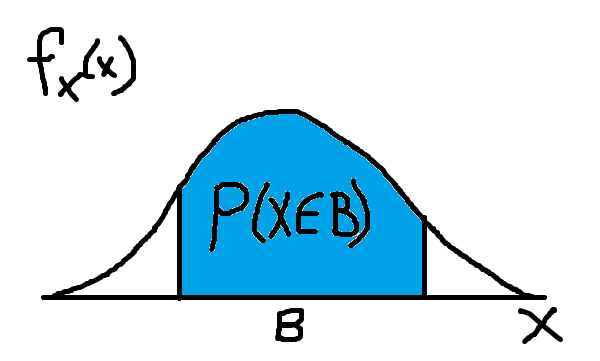
\includegraphics[width=100mm]{12.png}
	\caption{Illustration of $P(X\in B)$}
\end{figure}

The function $f_X(x)$ is known as a probability density function PDF of $X$. It can be obtained as a derivative of CDF:

$$f_X(x)=\frac{d}{dx}F_X(x)$$

given that $F_X(x)$ is continuous and differentiable everywhere. The requirements for $f_X(x)$ include

\begin{enumerate}[i]
	\item $f_X(x) \ge 0$ for all $x$
	\item $f_X(x)$ must be (piecewise) continuous for all $x$
	\item $\displaystyle \int_{-\infty}^\infty f_X(x) dx = 1$
\end{enumerate}

$f_X(x)$ can have $f_X(x)>1$ for some $x$ values since it is not a probability function. The CDF of $X$ can be readily obtained by

$$F_X(a)=P(X\le a)=\int_{-\infty}^a f_X(x) dx$$

The probability of a continuous random variablele $X$ in range $(a,b)$ is

$$P(a < X < b)=P(a \le X < b)=P(a < X \le b)=P(a \le X \le b)=\int_a^b f_X(x) dx = F_X(b)-F_X(a)$$

It follows that the probability of $X$ takes any specific $a$ value is

$$P(X=a)=\int_{a}^a f_X(x) dx=0$$

Note that even though the probability is zero, it is still possible for $X$ to take $a$. This is because $X$ can take infinitely many values in range $(-\infty,\infty)$ which makes the size of sample space infinite. The probability of landing on a specific $a$ in this infinite sample space is very very low so the probability is zero but it does not make it impossible. \\

We will look over some special continuous random variables.

\subsubsection{Continuous Uniform Random Variable}

A continuous uniform distribution random variable $X\sim \Unif(a, b)$ over the interval $[a,b]$ is described by the following PDF

$$
f_X(x)=\begin{cases}
	c & a \le x \le b \\
	0 & \text{otherwise}
\end{cases}
$$

where $c$ is some normalization constant. We can calculate it by follows:

\[\int_a^b cdx=c(b-a)=1\]

which gives $c=\frac{1}{b-a}$.

\begin{figure}[H]
	\centering
	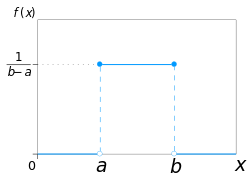
\includegraphics[width=100mm]{13.png}
	\caption{PDF for Continuous Uniform Distribution}
\end{figure}

It can be used to model outcomes that lie in some boundary. The total probability is $1$ as expected because the area of the rectangular region is

$$(b-a)\frac{1}{b-a}=1$$

Its CDF can be calculated by

\[F_X(x)=P(X\le x)=\int_{-\infty}^x f_X(x) dx = \int_a^x \frac{1}{b-a} dx = \frac{x-a}{b-a}\]

for $x\in[a,b]$. The full CDF for this distribution is:

\[F_X(x)=\begin{cases} 0 & x<a \\ \frac{x-a}{b-a} & a\le x \le b \\ 1 & x>b \end{cases}\]

\subsubsection{Exponential Random Variable}

An exponential random variable $X\sim\Exp(\lambda)$ of parameter $\lambda$ is described by the PDF

$$
f_X(x)=\begin{cases}
	\lambda  e^{-\lambda x} & x \ge 0 \\
	0 & x < 0
\end{cases}
$$

\begin{figure}[H]
	\centering
	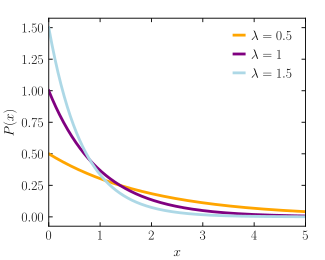
\includegraphics[width=100mm]{14.png}
	\caption{PDF for Exponential Distribution}
\end{figure}

This distribution is often used to find waiting times for periodic events. As an example suppose in a certain country (Japan I think), there is an earthquake that happens every ten years. Define $\lambda$ (in fact it is the same one used in Poisson's) as the number of earthquakes happening every year which is $\lambda=\frac{1}{10}$. Let the random variable $X$ denote waiting time in years. The probability that the earthquake happens in less than five years is

$$P(X\le5)=\int_0^5\lambda e^{-\lambda x}dx=0.393$$

and the probability that you need to wait more than a year to see the earthquake happen is

$$P(X>1)=1-P(X\le1)=1-\int_0^1\lambda e^{-\lambda x}dx=0.9048$$

Note that you can calculate the same probability using a Poisson random variable with the same parameter. Redefine $X$ as the number of earthquakes happening in a one-year timespan. The probability that there are no earthquakes in one year is

$$P(X=0)=e^{-\lambda}=0.9048$$

It gives the same result! An exponential distribution's ``waiting time'' does not have any events happening, hence in the Poisson distribution we set the number of events happening in that time period to zero $X=0$. \\

The other applications of exponential distributions include finding the half-life of radioactive material. These problems can be modelled as finding time $a$ such that

$$P(X\ge a)=\frac12$$

$a$ can be found by

$$e^{-\lambda a}=\frac12$$

which gives $a=\frac{\ln(2)}{\lambda}$. \\

The total probability of the exponential distribution is indeed one:

$$\int_{-\infty}^\infty f_X(x) dx = \int_0^\infty \lambda e^{-\lambda x} dx = \left. -e^{-\lambda x} \right\vert_0^\infty = 1$$

Exponential distributions also have memoryless property like geometric random variables. The waiting time for a future event does not depend on elapsed time:

$$P(X\ge s+t \mid X\ge s)=P(X\ge t)$$

\begin{proof}
	Evaluating $P(X\ge t)$ gives
	
	$$P(X\ge t)=\int_t^\infty \lambda e^{-\lambda x} dx = \left. -e^{-\lambda x} \right\vert_t^\infty = e^{-\lambda t}$$
	
	It also follows that
	
	$$P(X\ge s)=e^{-\lambda s} \quad P(X\ge s+t)=e^{-\lambda (s+t)}$$
	
	Using the definition of conditional probability to calculate $P(X\ge s+t \mid X\ge s)$ gives
	
	$$P(X\ge s+t \mid X\ge s)=\frac{P(X\ge s+t)}{P(X\ge s)}=\frac{e^{-\lambda (s+t)}}{e^{-\lambda s}}=e^{-\lambda t}$$
	
	this is the same as $P(X\ge t)$ which concludes the proof.
\end{proof}

As a supplement, we will show how Poisson distribution is used to derive exponential distribution. Let $X$ denote number of years. We saw earlier in the earthquake example that the probability that no earthquakes happen in one year is $e^{-\lambda}$. Now the probability that no earthquakes happen in $x$ years is just

$$P(X>x)=\underbrace{e^{-\lambda}e^{-\lambda}\cdots e^{-\lambda}}_{\text{$x$ times}}=e^{-\lambda x}$$

This allows us to define exponential distribution's CDF which is given by

$$F_X(x)=P(X\le x)=1-P(X>x)=1-e^{-\lambda x}$$

Finally we obtain exponential PDF by differentiating the CDF:

$$f_X(x)=\frac{d}{dx}F_X(x)=\lambda e^{-\lambda x}$$

\subsubsection{Normal Random Variable}

A normal random variable $X\sim \Norm(\mu,\sigma^2)$ of mean $\mu$ and variance $\sigma^2$ is described by the following PDF:

$$f_X(x)=\frac{1}{\sigma\sqrt{2\pi}}\exp\left(-\frac12 \left( \frac{x-\mu}{\sigma} \right)^2\right)$$

It produces the famous bell curve

\begin{figure}[H]
	\centering
	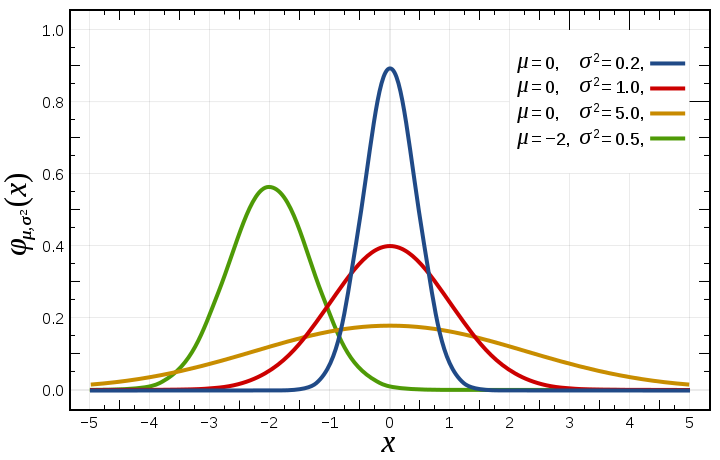
\includegraphics[width=100mm]{15.png}
	\caption{Normal PDF. $\mu$ specifies the center of mass of the distribution and $\sigma^2$ controls how wide the curve is. Bigger the $\sigma^2$ is, more flatter the curve becomes.}
\end{figure}

\begin{figure}[H]
	\centering
	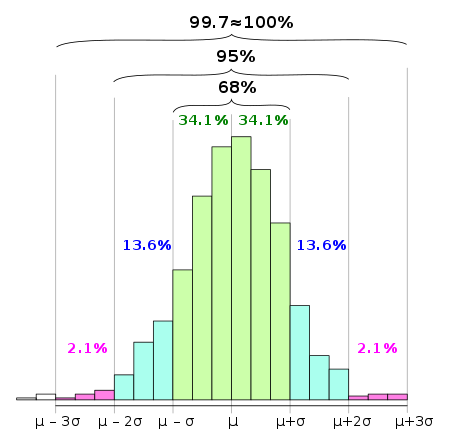
\includegraphics[width=120mm]{16.png}
	\caption{Distribution of mass in Gaussian. One standard derivation $\sigma$ left and right from mean value $\mu$ will give about $68\%$ of the overall mass. Two standard derivations left and right from the mean will give about $95\%$ of the overall mass.}
\end{figure}

Like other distributions, the total probability of this distribution is indeed one.

\begin{proof}
	\begin{align*}
		\int_{-\infty}^\infty f_X(x) dx &= \frac{1}{\sigma\sqrt{2\pi}} \int_{-\infty}^\infty \exp\left(-\frac12 \left( \frac{x-\mu}{\sigma} \right)^2\right) dx
		\intertext{Change of variables using $t=x-\mu$ gives}
		&= \frac{1}{\sigma\sqrt{2\pi}} \int_{-\infty}^\infty \exp\left(-\frac{t^2}{2\sigma^2} \right) dt
	\end{align*}
	
	Denote the integral $\int_{-\infty}^\infty \exp\left(-\frac{t^2}{2\sigma^2} \right) dt$ by $I$. Integrating $I^2$ gives
	
	\begin{align*}
		I^2 &= \int_{-\infty}^\infty \exp\left(-\frac{x^2}{2\sigma^2} \right) dx \int_{-\infty}^\infty \exp\left(-\frac{y^2}{2\sigma^2} \right) dy \\
		&= \int_{-\infty}^\infty \int_{-\infty}^\infty \exp\left(-\frac{x^2}{2\sigma^2} -\frac{y^2}{2\sigma^2} \right) dx dy
		\intertext{We switch to polar coordinates}
		&= \int_{0}^\infty \int_{0}^{2\pi} \exp\left(-\frac{r^2}{2\sigma^2} \right) r d\theta dr \\
		&= 2\pi \int_{0}^\infty \exp\left(-\frac{r^2}{2\sigma^2} \right) rdr
		\intertext{We make another change of variables using $u=\frac{r^2}{2\sigma^2}$ which gives}
		&= 2\pi \int_0^\infty e^{-u} \sigma^2 du \\
		&= 2\pi \sigma^2
	\end{align*}
	
	This gives $I=\sigma\sqrt{2\pi}$. Now
	
	\begin{align*}
		\int_{-\infty}^\infty f_X(x) dx = \frac{1}{\sigma\sqrt{2\pi}} I = \frac{1}{\sigma\sqrt{2\pi}} \sigma\sqrt{2\pi} = 1
	\end{align*}
\end{proof}

The CDF for normal distribution is 

$$F_X(a)=P(X\le a)=\frac{1}{\sigma\sqrt{2\pi}} \int_{-\infty}^a \exp\left(-\frac12 \left( \frac{x-\mu}{\sigma} \right)^2\right) dx$$

There is no closed-form expression for $F_X(a)$. However, we can define standard normal $\Norm(0, 1)$ whose PDF is

$$f_X(x)=\frac{1}{\sqrt{2\pi}}\exp\left(-\frac{x^2}{2}\right)$$

and its CDF is

$$\phi(x) = \frac{1}{\sqrt{2\pi}}\int_{-\infty}^x \exp\left(-\frac{x^2}{2}\right) dx$$

Standard normal's CDF $\phi(x)$\footnote{In terms of error round function $\text{erf}$, $\phi$ can be written as $\phi(x)=\frac{1+\text{erf}(x/\sqrt{2})}{2}$.} can be used to calculate $F_X(a)$:

$$F_X(a)=\phi\left( \frac{a-\mu}{\sigma} \right)$$

\begin{figure}[H]
	\centering
	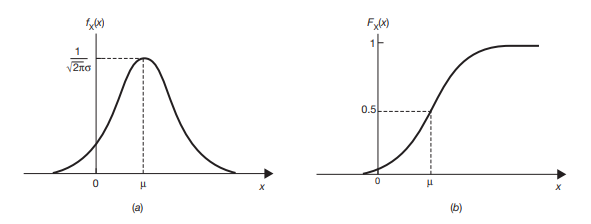
\includegraphics[width=120mm]{17.png}
	\caption{Standard Normal's PDF and CDF}
\end{figure}

Normal random variable $X\sim \Norm(\mu,\sigma^2)$ can be scaled to standard normal $Z\sim \Norm(0,1)$ with $Z=\frac{X-\mu}{\sigma}$.

\begin{proof}
	The probability of $Z\le t$ is
	
	$$P(Z\le t)=\frac{1}{\sqrt{2\pi}}\int_{-\infty}^t \exp\left(-\frac{z^2}{2}\right) dz \quad\star$$
	
	Since $X=\sigma Z+\mu$, $Z\le t$ is same as $X\le \sigma t+\mu$. So the probability of $X\le \sigma t+\mu$ is
	
	$$P(X\le \sigma t+\mu)=\frac{1}{\sigma\sqrt{2\pi}} \int_{-\infty}^{\sigma t+\mu} \exp\left(-\frac12 \left( \frac{x-\mu}{\sigma} \right)^2\right) dx$$
	
	Change of variables using $z=\frac{x-\mu}{\sigma}$\footnote{In statistics, $z$ is known as ``z-score.'' It measures how far $x$ deviates from mean $\mu$ in units of $\sigma$.} will convert this integral to the one marked with $\star$.
\end{proof}

Normal distributions have a broad range of applications everywhere. It is often used for random variables with unknown distribution patterns.

\begin{texample}
	A group of programmers is trying to fix a buggy random number generator. They found that the mean of all generated random numbers is $310$ with standard deviation is $23$. What is the probability that it will generate a number somewhere between $250$ and $300$? \\
	
	Let the normal random variable $X\sim \Norm(310, 23^2)$ denote the random number generated. We want to calculate $P(250\le X\le 300)$. We can simplify the calculation using this substitution $Z=\frac{X-\mu}{\sigma}$ so the probability can be looked up using a standard normal table.
	
	$$P(250\le X\le 300) = P(\frac{250-310}{23} \le \frac{X-\mu}{\sigma} \le \frac{300-310}{23}) = P(-2.61 \le Z \le -0.43)$$
	
	Since the normal distribution is symmetric, $P(-2.61 \le Z \le -0.43)$ is same as $P(0.43 \le Z \le 2.61)$. The probability is
	
	$$P(0.43 \le Z \le 2.61)=P(0 \le Z \le 2.61) - P(0 \le Z \le 0.43) \approx 0.4955 - 0.1664=0.3291$$
\end{texample}

\begin{texample}
	A prisoner plays with a laser pointer in his jail cell. He randomly directs the laser beam at the wall one meter away from him.
	
	\begin{figure}[H]
		\centering
		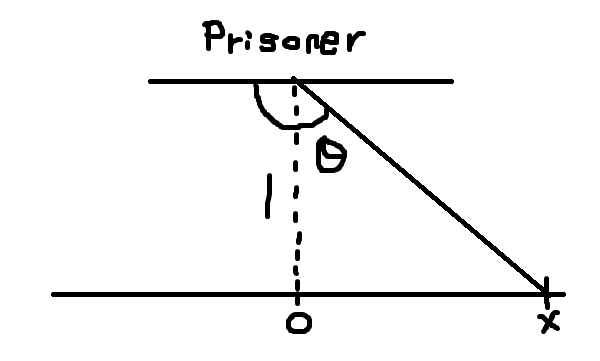
\includegraphics[width=80mm]{18.png}
		\caption{Prisoner Playing with Laser}
	\end{figure}
	
	The laser beam angle $\theta$ is uniform in $[0, \pi]$. A security guard wants to find the most likely distance $x$ from origin $O$ where the laser beam lands. \\
	
	Let random variable $X$ denote the distance from the origin. We need to find CDF for $X$:
	
	$$F_X(x)=P(X\le x)$$
	
	We can calculate $P(X\le x)$ using geometry. $x$ is some arbitrary distance from origin. From the diagram when the laser beam hits $x$, its angle is $\arctan x+\frac{\pi}{2}$. When $X\le x$, it follows that the angle $\theta \le \arctan x+\frac{\pi}{2}$. The probability that $X\le x$ is:
	
	$$P(X\le x)=P(\theta \le \arctan x+\frac{\pi}{2})=\frac{1}{\pi}\left( \arctan x+\frac{\pi}{2} \right)=\frac{1}{\pi}\arctan x+\frac12$$
	
	The PDF for $X$ can be obtained by differentiating $F_X(x)$:
	
	$$f(x)=\frac{d}{dx}F_X(x)=\frac{1}{\pi (1+x^2)}$$
	
	This is also the PDF for the standard Cauchy distribution.
	
	\begin{figure}[H]
		\centering
		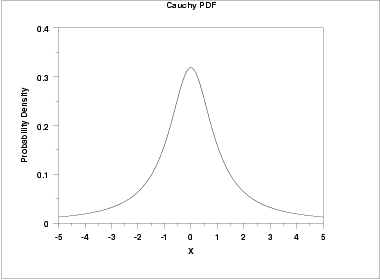
\includegraphics[width=100mm]{19.png}
		\caption{Standard Cauchy PDF}
	\end{figure}
	
	The laser beam will most likely hit somewhere around $x=0$.
\end{texample}

\subsubsection{Expectation Value}

For continuous random variables $X$ with PDF $f(x)$, its expectation is defined as

$$E[X]=\int_{-\infty}^\infty xf(x) dx$$

Expectation for continuous uniform random variables can be calculated as follows:

$$E[X\sim \Unif(a,b)]=\int_{-\infty}^\infty xf(x) dx=\int_a^b \frac{x}{b-a} dx=\frac{a+b}{2}$$

For exponential random variables, straightforward integration by parts gives

\begin{align*}
	E[X\sim\Exp(\lambda)]&=\int_0^\infty x\lambda e^{-\lambda x} dx \\
	&=\left. -xe^{-\lambda x} \right\vert_0^\infty + \int_0^\infty e^{-\lambda x} dx \\
	&=\frac{1}{\lambda}
\end{align*}

For normal random variables,

$$E[X\sim \Norm(\mu, \sigma^2)]=\mu$$

I leave the calculation details for the readers. \\

\subsection{More on Expectation}

\begin{theorem}
	If a continuous random variable $X \ge 0$, then
	
	\[ EX=\int_0^\infty P(X\ge t) dt \]
\end{theorem}

\begin{proof}
	\[ EX = \int_0^\infty P(X\ge t) dt = \int_0^\infty 1-F_X(t) dt \]
	
	where $F_X(t)$ is CDF of $X$. Integrating by parts using $u=1-F_X(t)$ and $dv=dt$ gives
	
	\[ EX = \left. t (1-F_X(t)) \right\vert_0^\infty + \int_0^\infty t f_X(t) dt \]
	
	where $f_X(t)=\frac{d}{dt}F_X(t)$ is PDF for $X$. Provided that $\lim_{t\to\infty} t (1-F_X(t)) = 0$, we are left with
	
	\[ EX = \int_0^\infty t f_X(t) dt \]
\end{proof}

If $X$ is a discrete random variable that takes values $0, 1, 2, \dots$,

\[ EX=\sum_{a=0}^\infty P(X>a) \]

\begin{theorem}
	Law of the Unconscious Statistician: Let $g : \mathbb{R} \to \mathbb{R}$ be an only function and $X$ is a continuous random variable, then $g(X)$ is a new random variable. It follows that the expectation value for $g(X)$ is
	
	\[ Eg(X)=\int_{-\infty}^\infty g(x) f(x) dx \]
	
	If $X$ is discrete random variable,
	
	\[ Eg(X)=\sum_i g(x_i) p(x_i) \]
\end{theorem}

\begin{proof}
	If $g \ge 0$ then $g(X)\ge0$. The expectation for $g(X)$ is
	
	\[ Eg(X)=\int_0^\infty P(g(x)\ge t) dt \]
	
	Define a set $B_t=\{ x : g(x)\ge t \}$,
	
	\[ Eg(X)=\int_0^\infty \int_{B_t} f(x) dx \: dt \]
	
	\begin{figure}[H]
		\centering
		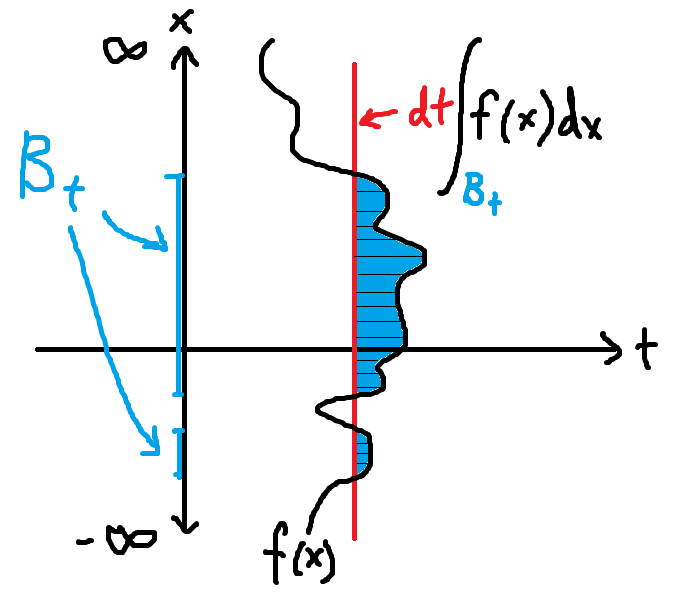
\includegraphics[width=100mm]{20.png}
		\caption{Visualization of the integral $\displaystyle\int_0^\infty \int_{B_t} f(x) dx \: dt$}
	\end{figure}
	
	Changing the integration order gives
	
	\[ Eg(X)=\int_{-\infty}^\infty \int_0^{g(x)} f(x) dt \: dx = \int_{-\infty}^\infty g(x) f(x) dx \]
\end{proof}

There is an important special case to consider: Let $a$ and $b$ denote constants. Suppose $g(X)=aX+b$,

\[ E(aX+b)=\int (ax+b)f(x)dx=a\int xf(x)dx+b\int f(x) dx = aEX+b \]

(The whole integral of the PDF is one: $\int_{-\infty}^\infty f(x) dx=1$.) This shows that expectation is linear.

\begin{texample}
	A particle of mass 1g has a random velocity $X$ that is uniformly distributed between 3cm/s and 8cm/s. Find the probability density of the particle's kinetic energy $T=\frac12X^2$. Find the mean of $T$ in two ways: using the PDF for $T$ and the Law of the Unconscious Statistician. \\
	
	$X$ is a continuous uniform random variable with the following CDF:
	
	\[F_X(x)=P(X\le x)=\begin{cases} 0 & x<3 \\ \frac{x-3}{5} & 3\le x \le8 \\ 1 & x>8 \end{cases}\]
	
	The CDF for $T$ is:
	
	\[F_T(t)=P(T\le t)=P\left(\frac12X^2\le t\right)=P(X\le\sqrt{2t})=\begin{cases} 0 & t<\frac92 \\ \frac{\sqrt{2t}-3}{5} & \frac92\le t \le32 \\ 1 & t>32 \end{cases}\]
	
	The PDF for $T$ is:
	
	\[f_T(t)=\frac{d}{dt}F_T(t)=\begin{cases} 0 & t<\frac92 \\ \frac{1}{5\sqrt{2t}} & \frac92\le t \le32 \\ 1 & t>32 \end{cases}\]
	
	The mean for $T$ is using the PDF directly is:
	
	\[ET=\int_{\frac92}^{32} t\frac{1}{5\sqrt{2t}} dt=\frac{97}{6}\]
	
	or using the Law of the Unconscious Statistician:
	
	\[ET=E[\frac12X^2]=\int_3^8 \left( \frac12x^2 \right)\frac{1}{5}dx=\frac{97}{6}\]
	
	They both give the same answer!
\end{texample}

\begin{texample}
	Stanislaw is collecting coupons. Each day he receives randomly one of $n$ distinct coupons with equal probabilities (independently of other days). Let $T$ be the number of days it takes Stanislaw to obtain a complete set. Compute the expected value of $T$. \\
	
	Let $T_i$ be the number of days until Stanislaw has $i$ different coupons. We let $T_0 = 0$, and clearly $T_1 = 1$. We are interested in $T = T_n$. Let $X_i = T_i-T_{i-1}$, so $T = X_1+X_2+\cdots+X_n$. Once Stanislaw has $i-1$ coupons, each day there is probability $\frac{n-i+1}{n}$ of getting a new coupon. These attempts to get a new coupon are independent until the next success, so $X_i\sim\Geom\left( q \right)$ with parameter $q=\frac{n-i+1}{n}$. The expectation for $T$ is
	
	\[E[T]=\sum_{i=1}^n E[X_i]=\sum_{i=1}^n \frac{n}{n-i+1} \approx n\log n\]
\end{texample}

\subsection{Moment and Variance}

The nth moment of a random variable $X$ is defined as

\[ E(X^n)=\begin{cases} \displaystyle\int_{-\infty}^\infty x^n f(x) dx & \text{$X$ continuous} \\[20pt] \displaystyle\sum_i x_i^n p(x_i) & \text{$X$ discrete} \end{cases} \]

Note that $E(X^n) = (EX)^n$ is not true all the time. From the definition, it follows that mean $EX$ is the first moment of $X$. $EX$ is usually denoted by $\mu$. \\

The variance (or second central moment) of $X$ is defined as

\[ \Var(X)=\sigma^2=E((x-\mu)^2) \]

$\Var(X)$ is always greater than or equal to zero. The standard deviation is just the square root of variance: $\sigma=\sqrt{\Var(X)}$. They both measure the spread of distribution from the mean. \\

Note that the following is equivalent

\[ \Var(X)=E(X^2)-(EX)^2 \]

\begin{proof}
	\begin{align*}
		\Var(X)&=E((x-\mu)^2) \\
		&=E(x^2-2x\mu+\mu^2) \\
		&=\int (x^2-2x\mu+\mu^2) f(x) dx \\
		&=\int x^2 f(x) dx -2\mu\int xf(x) dx + \mu^2 \int f(x) dx \\
		&=E(X^2)-2\mu EX + \mu^2 \\
		&=E(X^2)-2(EX)^2+(EX)^2 \\
		&=E(X^2)-(EX)^2
	\end{align*}
\end{proof}

Variances for some random variables are given in the below table

\begin{center}
	\begin{tabular}{| c | c |}
		\hline
		Random variable $X$ & $\Var(X)$ \\
		\hline
		$\Bin(n,p)$ & $np(1-p)$ \\
		\hline
		$\Pois(\lambda)$ & $\lambda$ \\
		\hline
		$\Exp(\lambda)$ & $\frac{1}{\lambda^2}$ \\
		\hline
		$\Norm(\mu,\sigma^2)$ & $\sigma^2$ \\
		\hline
	\end{tabular}
\end{center}

\begin{theorem}
	Let $a$ and $b$ denote constants,
	
	\[ \Var(aX+b)=a^2\Var(X) \]
	
	or variance is independent of $b$ added to $X$ (ie. invariant of location) and if $X$ is scaled by $a$, variance is scaled by $a^2$.
\end{theorem}

\begin{proof}
	First, we prove that $\Var(X+b)=\Var(X)$,
	
	\begin{align*}
		\Var(X+b)&=E((X+b)^2)-(E(X+b))^2
		\intertext{Since expectation is linear operator: $E(X+b)=EX+b$,}
		&=E(X^2+2bX+b^2)-(EX+b)^2 \\
		&=E(X^2)+2b(EX)+b^2-((EX)^2+2b(EX)+b^2) \\
		&=E(X^2)+2b(EX)+b^2-(EX)^2-2b(EX)-b^2 \\
		&=E(X^2)-(EX)^2 \\
		&=\Var(X)
	\end{align*}
	
	Next, we prove that $\Var(aX)=a^2\Var(X)$,
	
	\begin{align*}
		\Var(aX)&=E((aX)^2)-(E(aX))^2 \\
		&=a^2E(X^2)-a^2(EX)^2 \\
		&=a^2(E(X^2)-(EX)^2) \\
		&=\Var(X)
	\end{align*}
\end{proof}
